\documentclass[12pt,a4paper]{report}
\usepackage[utf8]{inputenc}
\usepackage[T1]{fontenc}
\usepackage{lmodern}
\usepackage{caption}
\captionsetup{font=footnotesize}
\usepackage{amsmath}
%\usepackage{algorithm}
\usepackage{listings}
%\usepackage{standalone}
%\usepackage{algpseudocode}
\usepackage[linesnumbered,lined,boxed,commentsnumbered]{algorithm2e}
\SetKw{KwBy}{by} 
\newcommand\mycommfont[1]{\footnotesize\ttfamily{#1}}
\SetCommentSty{mycommfont}
\usepackage{verbatim}
\usepackage{tabularx}
%\usepackage{program}
%\input{externaldoc}
%\input{verticalblock}
%\algrenewcommand\algorithmicindent{1.0em}
\usepackage{minitoc}
\usepackage{float}
\usepackage{hyperref}
\usepackage{physics}
\usepackage{color}
\usepackage{subfiles}
\usepackage{pdfpages}
\usepackage{centernot}
\usepackage[ED=SDM-PMat, Ets=UT3]{tlsflyleaf}

\hypersetup{
 colorlinks=true,
 linkcolor=blue,
 filecolor=blue,
 urlcolor=blue,
 citecolor=blue
}
\usepackage{mathpazo,libertine}



\newcommand{\alert}[1]{\textcolor{red}{#1}}
\newcommand{\Hij}[3][\hat{H}]{\mel{#2}{#1}{#3}}
%\newcommand{\ket}[1]{| #1 \rangle}

%sizes
\newcommand{\Ndet}{{N_\text{det}}}
\newcommand{\Ngen}{{N_\text{gen}}}
\newcommand{\Nsel}{{N_\text{sel}}}
\newcommand{\Norb}{{N_\text{orb}}}
\newcommand{\Nelec}{{N_\text{elec}}}
\newcommand{\Nalpha}{{N_\text{elec}^\alpha}}
\newcommand{\Nbeta}{{N_\text{elec}^\beta}}
\newcommand{\Nint}{{N_\text{int}}}
\newcommand{\Nst}{{N_\text{states}}}
\newcommand{\Ndav}{{N_\text{dav}}}
\newcommand{\Nperm}{{N_\text{perm}}}
\newcommand{\Na}{{N_\alpha}}
\newcommand{\Nb}{{N_\beta}}
\newcommand{\Ne}{{N_\text{elec}}}
\newcommand{\NFCI}{N_\text{FCI}}

%bitmasks
\newcommand{\bit}[1]{{\texttt{#1}}}
\newcommand{\bitI}{{\texttt{I}}}
\newcommand{\bitP}{{\texttt{P}}}
\newcommand{\bitJ}{{\bit{J}}}
\newcommand{\bitK}{{\bit{K}}}
\newcommand{\bitx}[2]{{\texttt{#1}_{#2}}}
\newcommand{\bitIsigma}{{\bitx{I}{\sigma}}}
\newcommand{\bitPsigma}{{\bitx{P}{\sigma}}}
\newcommand{\binary}[1]{{#1_{\mathtt{2}}}}
\newcommand{\TRUE}{{\text{\texttt{TRUE}}}}
\newcommand{\FALSE}{{\text{\texttt{FALSE}}}}


%acronyms
\newcommand{\HF}{{\text{HF}}}
\newcommand{\QP}{{ \textsc{Quantum Package} }}

%energies
\newcommand{\EDMC}{E_\text{DMC}}
\newcommand{\EPT}{E_\text{PT2}}
\newcommand{\Ecor}{E_\text{corr}}
\newcommand{\Evar}{E_\text{var}}
\newcommand{\EFCI}{E_\text{FCI}}
\newcommand{\ECI}{E_\text{CI}}
\newcommand{\E}[1]{E_{#1}}


%operators
\newcommand{\vac}{ {\ket{}} }
\newcommand{\ac}[1]{a^\dagger_{#1}}
\newcommand{\an}[1]{a_{#1}}
\newcommand{\hH}{\Hat{H}}
\newcommand{\ordering}{{\hat{\mathcal{O}}}}
\newcommand{\phase}[2]{{\Phi \qty(#1 \rightarrow #2)}}

%determinants
\newcommand{\kalpha}{{\ket{\alpha}}}
\newcommand{\kbeta}{{\ket{\beta}}}
\newcommand{\ki}{{\ket{i}}}
\newcommand{\kj}{{\ket{j}}}
\newcommand{\kI}{{\ket{I}}}
\newcommand{\kIp}{{\ket{I'}}}
\newcommand{\kJ}{{\ket{J}}}
\newcommand{\kJp}{{\ket{J'}}}
\newcommand{\kK}{{\ket{J}}}
\newcommand{\occ}[2]{{\text{occ}(#1,#2)}}

%excitation
\newcommand{\excdet}[2]{{\hat{T}_{#1 \rightarrow #2}}}
\newcommand{\excorb}[2]{{\hat{T}_{#1}^{#2}}}

%space
\newcommand{\br}{{\mathbf{r}}}
\newcommand{\bR}{{\mathbf{R}}}

%Fortran
\newcommand{\POPCNT}[1]{\text{\texttt{POPCNT}}(#1)}
\newcommand{\TRAILZ}[1]{\text{\texttt{TRAILZ}}(#1)}
\newcommand{\IBSET}[1]{\text{\texttt{IBSET}}(#1)}
\newcommand{\IBCLR}[2]{\text{\texttt{IBCLR}}(#1,#2)}
\newcommand{\BTEST}[2]{\text{\texttt{BTEST}}(#1,#2)}
\newcommand{\ISHFT}[2]{\text{\texttt{ISHFT}}(#1,#2)}
\newcommand{\IAND}[2]{\text{\texttt{IAND}}(#1,#2)}
\newcommand{\IEOR}[2]{\text{\texttt{IEOR}}(#1,#2)}
\newcommand{\IOR}[2]{\text{\texttt{IOR}}(#1,#2)}
\newcommand{\NOT}[1]{\text{\texttt{NOT}}(#1)}

\newcommand{\popcnt}[1]{\norm{#1}}
\newcommand{\trailz}[1]{\text{trailing\_zeros}(#1)}
\newcommand{\ibset}[1]{\text{bit\_set}(#1)}
\newcommand{\ibclr}[2]{\text{bit\_clear}(#1,#2)}
\newcommand{\btest}[2]{\text{bit\_test}(#1,#2)}
\newcommand{\ishft}[2]{\text{shift\_left}(#1,#2)}
\newcommand{\iand}[2]{#1 \wedge #2}
\newcommand{\ieor}[2]{#1 \oplus #2}
\newcommand{\ior}[2]{#1 \vee #2}
%\newcommand{\not}[1]{{\neg #1}}

%Sets
\newcommand{\set}[1]{{\mathcal{#1}}}
\newcommand{\setx}[2]{{\mathcal{#1}_{#2}}}
\newcommand{\setI}{\set{I}}
\newcommand{\setJ}{\set{J}}

%matrices and vectors
\newcommand{\mH}{\mathbf{H}}
\newcommand{\mc}{\mathbf{c}}



%centering in tables
\newcommand{\tabc}[1]{\multicolumn{1}{c}{#1}}




%%%%%
% À mettre dans le préambule (avant \begin{document})
%%%%%
%% Titre, auteur, date, laboratoire, cotutelle
%\title{Development and parallel implementation of Selected Configuration Interaction methods}
\title{Développement et implémentation parallèle de méthodes d'interaction de configurations sélectionnées}
\author{Yann GARNIRON}
\defencedate{15/11/2018}
\lab{Laboratoire de Chimie et Physique Quantiques (UMR 5626)}
%\cotutelle{Institut de cotutelle}

%% Directeur(s) de thèse
\nboss{1}                                    % Nombre de directeur(s) de thèse
\makesomeone{boss}{1}{Anthony SCEMAMA}{Ingénieur de Recherche}{Directeur} % Sera affiché en premier
%% Referee
\nreferee{2}
\makesomeone{referee}{1}{Philippe CARBONNIERE}{Professeur d'Université}{Rapporteur}
\makesomeone{referee}{2}{Jean-Philip PIQUEMAL}{Professeur d'Université}{Rapporteur}
%% Jury
\njudge{2}
\makesomeone{judge}{1}{Nathalie GUIHERY}{Professeure d'Université}{Président du Jury}
\makesomeone{judge}{2}{Nicolas RENON}{Ingénieur de Recherche}{Examinateur}
%\makesomeone{judge}{3}{Troisième MEMBRE}{Chargé de Recherche}{}


\usepackage[square,sort,comma,numbers]{natbib}
\usepackage{graphicx}


\lstset{% setup listings
        language=Fortran,% set programming language
        basicstyle=\ttfamily\footnotesize,% basic font style
%       keywordstyle=\bfseries,% keyword style
%        commentstyle=\ttfamily\itshape,% comment style
%       numbers=left,% display line numbers on the left side
%       numberstyle=\scriptsize,% use small line numbers
%       numbersep=10pt,% space between line numbers and code
        tabsize=2,% sizes of tabs
        showstringspaces=false,% do not replace spaces in strings by a certain character
        captionpos=b,% positioning of the caption below
        breaklines=true,% automatic line breaking
        escapeinside={(*}{*)},% escaping to LaTeX
        extendedchars=false,% prohibit extended chars (chars of codes 128--255)
        otherkeywords={assert,
            POPCNT, ISHFT, IBCLR, IOR, IEOR, TRAILZ, IAND, NOT, BTEST}
}



\begin{document}

\dominitoc

%\makeflyleaf
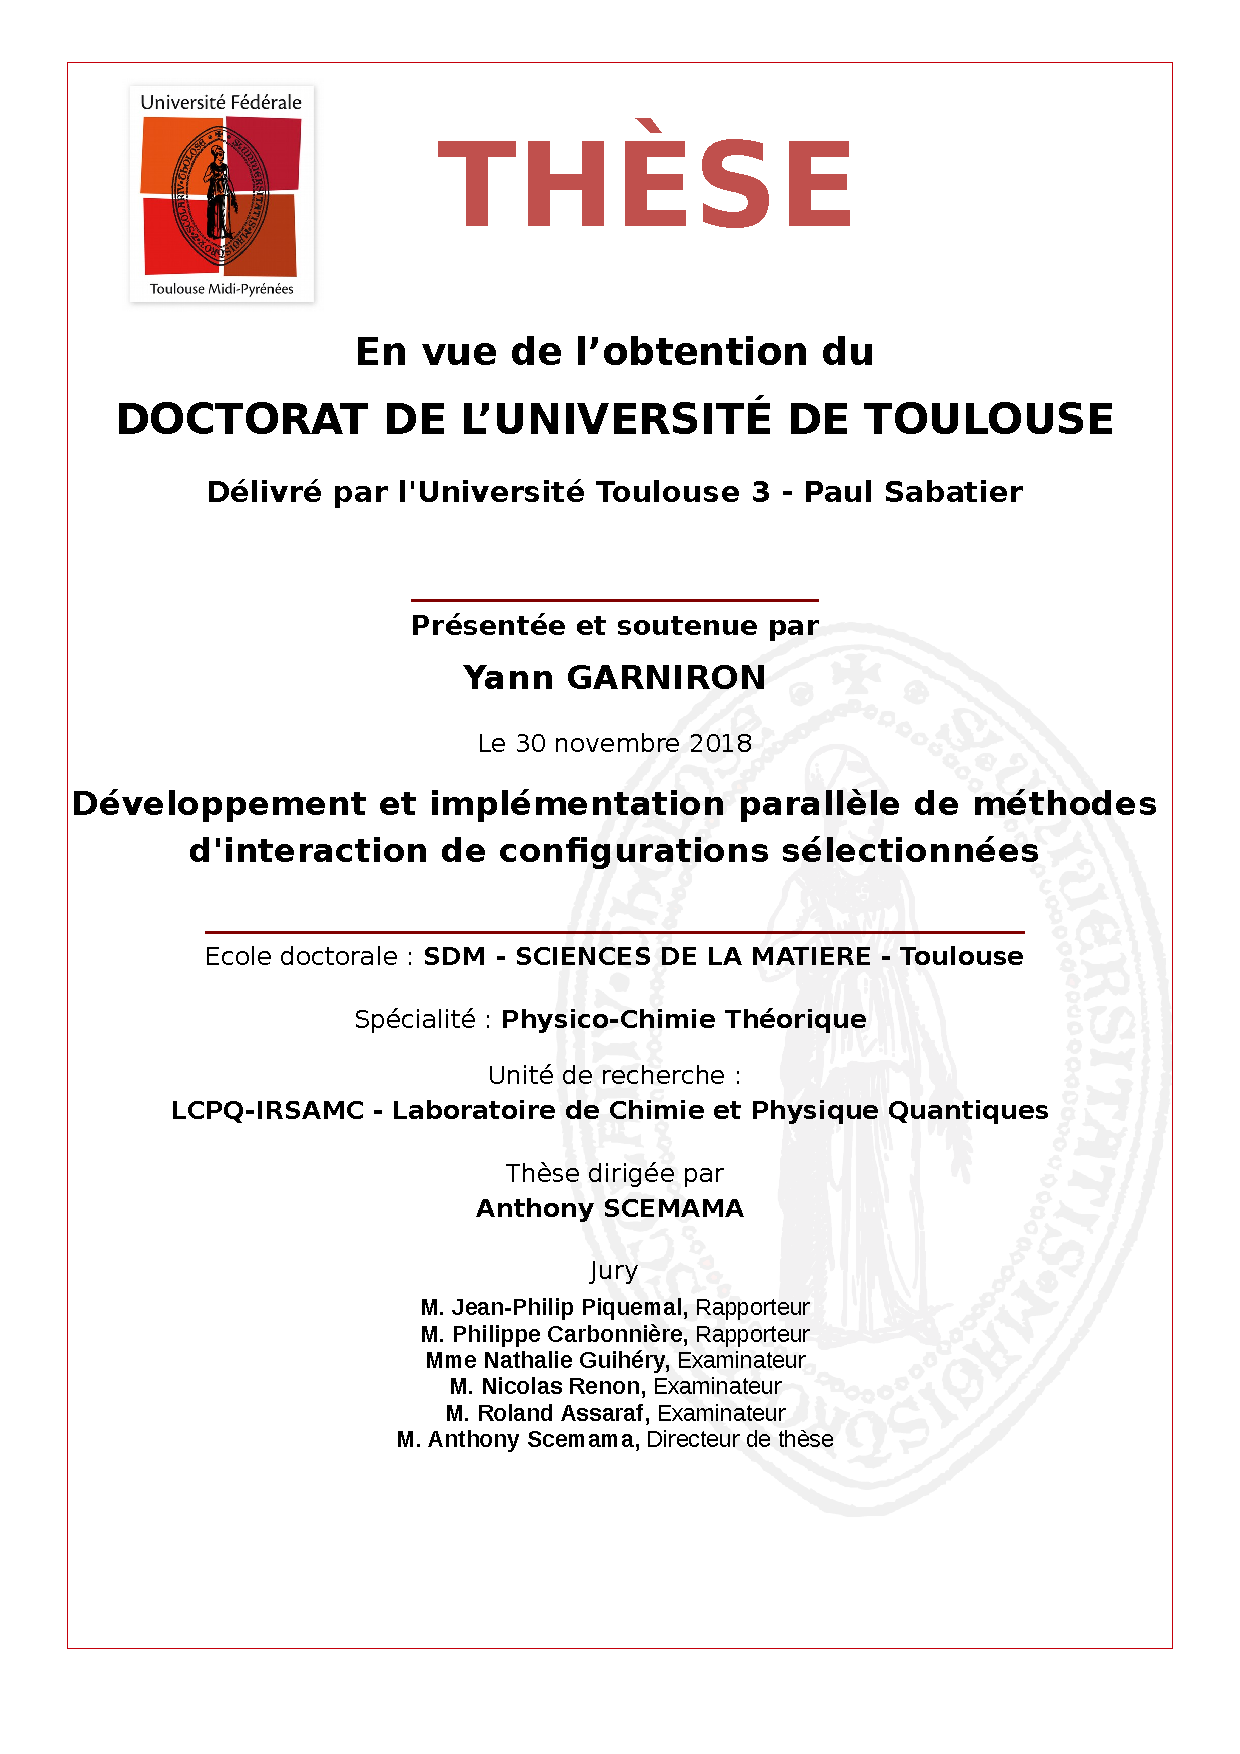
\includepdf{couverture_these}
\newpage

\chapter*{Acknowledgments - PROBLEMS}



%Alors?? Tu n'ecris pas ta these ???




\newpage

\tableofcontents
\newpage

\section*{Notations}

\begin{itemize}

\item [$\Norb$] Number of molecular orbitals

\item [$\Nst$] Number of considered eigenstates

\item [$\Ndet$] Number of determinants in the internal space

\item [$\Ngen$] Number of generator determinants 

\item [$\Nsel$] Number of selector determinants

\item [$\Nelec$] Number of electrons

\item [$\Nalpha$] Number of $\alpha$-spin electrons

\item [$\Nbeta$] Number of $\beta$-spin electrons

\item [$\Nint$] : Number of 64-bit integers required to store $\Norb$ bits : 
${\Nint = \lfloor \frac{\Norb-1}{64} \rfloor + 1}$

%\item [$\Ndav$] : Number of vectors in the Davidson diagonalization
%
%\item [$\Nperm$] : Number of permutations

\item [$\NFCI$] : Number of determinants in the FCI space

\item [$|\mathcal{D}|$] : Cardinality of the set $\mathcal{D}$.

\item [$\kalpha$] : external determinant
\end{itemize}


%centering in tables



\chapter{Introduction}

%During the 3 years I spent at the LCPQ, I worked on improving the \QP, a suit of quantum chemistry code intended for developers, which focuses on ease of implementation and parallelism.

Quantum chemistry is a discipline which relies on very expensive computations.
The scalings of wave function methods lie between $\order{N^5}$ and
$\order{N^8}$, where $N$ is proportional to the number of electrons in the
system. Therefore, performing accurate calculations requires both
approximations that can reduce the scaling, and an efficient implementation
that can take advantage of modern architectures. The work presented in this
thesis is more centered on this last aspect. 

In 1965, Gordon Moore predicted that the number of transistors in an integrated
circuit would double about every two years (the so-called Moore's
law).\cite{Moore}  Rapidly, this ``law'' was interpreted as an expected
$2\times$ gain in performance every 18 months, which became an industrial goal.
The development of today's most popular codes of the community
(Molpro\cite{Molpro}, Molcas\cite{Molcas}, or Gaussian\cite{g09}\dots) was
initiated in the 1990's.  At that time, the increase of computational power
from one generation of supercomputers to the next one was mostly due to the
increase of the frequency of the processors. the amount of random access memory
was small, the time to access data from disk was slow, and the energy
consumption of the most powerful computer was 236kW, which was not an
economical concern.\cite{top500_93}
At the beginning of the years 2000, having increased continuously both the number
of processors and their frequency raised the power consumption of
supercomputers by two orders of magnitude, raising accordingly the annual
electricity bill.  The only way to slow down this need for electricity while
keeping alive Moore's law was to keep the frequency fixed (between $1$ and
$4$~GHz), and increase the number of CPU cores.  The consequence of such a
choice was that ``free lunch'' was over, and the programmers now had to parallelize
their programs to make them run faster.\cite{Sutter_2005}
At the same time, computer scientists
realized that the increase of performance in memory access was slower than the
increase in computational power,\cite{Wulf1995Mar} and that the floating-point
operation (or flop) count would soon not be the bottleneck, and that data
movement would be the concern. This change was called the \emph{memory wall}.

So today, the situation is completely different from the 1990's.
Moore's law has ended,\cite{Khan2018Jan} the CPU frequency tends to decrease,
hundreds of thousands of cores need to be handled, data movement is the
principal concern, and disk access times are prohibitively high.
The work presented in this thesis is in the context of this change of paradigm
that has been going on for the last decade.
The traditional sequential algorithms of quantum chemistry are currently being
redesigned so as to be replaced by parallel equivalents by multiple groups
around the world, and this has also an influence on methodological development.

Initially, this work may been have expected to focus on methods that are by
design adapted to massively parallel architectures, such as Monte-Carlo methods
(stochastic methods), which are composed of a large number of independent tasks
(\emph{embarrassingly parallel} algorithms). In addition, they often are able
to yield a satisfactory result for just a fraction of the cost of the
equivalent deterministic, exact computation. An example of the move toward this
type of method is the recently developed \emph{Full Configuration Interaction
Quantum Monte Carlo} (FCIQMC).\cite{Booth_2009} FCIQMC can be interpreted as a
Monte-Carlo variant of older selected configuration interaction algorithms such as
CIPSI,\cite{Huron_1973} that are iterative and thus a priori not well adapted to
massively parallel architectures. But things turn out differently, and the
focus of this thesis was to investigate how to make \emph{configuration
interaction} (CI) methods efficient on modern supercomputers.
%Unlike Monte-Carlo, most wavefunction methods are not easy to parallelize.

The \QP developed at the LCPQ is a suite of wavefunction quantum
chemistry methods, that strives to allow easy implementation and
experimentation of new methods, and to make parallel computation
as simple and efficient as possible. The main purpose of this package
is to make experimentation on code design, algorithms and methods,
more than to be used massively in production.
Hence, the initial choice of the \QP was to go in the direction of
determinant-driven algorithms, as opposed to the more traditional
integral-driven algorithms.
A determinant-driven approach essentially implies that the wavefunction
is expressed as a linear combination of determinants, and that the 
outermost loops of the algorithms loop over determinants.
On the other hand, integral-driven algorithms have their outermost loop
on the two-electron integrals which appear in the expression of the matrix
elements in the determinant basis.
In the context of configuration interaction or perturbative
methods, the determinant-driven approach simplifies the development and allows
the researchers to test new ideas very quickly. These algorithms allow more
flexibility than their integral-driven
counterparts,\cite{Povill_1995} but they have been known for years to
be less efficient for solving problems that can be solved with an
integral-driven variant. High-precision calculations are in a regime
where the number of determinants is larger than the number of integrals,
which justifies the integral-driven choice.  Today, programming imposes
parallelism, and if
determinant-driven calculations prove to be better adapted to parallelism, such
methods could regain in popularity. The work presented in this thesis focuses
on determinant-driven approaches via the improvement of the \QP from
the methodological, algorithmic and the implementational points of views.


Somewhat logically, the first focus was the acceleration and parallelization of the
Davidson diagonalization, which is a pivotal point for CI methods.
A naive determinant-driven algorithm implies a quadratic scaling with the
number of determinants, while the integral-driven algorithm is expected to
scale linearly. This fact gave us some insight that there was room for
improvement in this step. 

The second focus was the improvement of the determinant selection algorithm
which is the main method used by the \QP to build compact wavefunctions
suitable for determinant-driven computations. In a nutshell, the principle is
to incrementally build a variational wavefunction by scavenging its external
space for determinants that interact with it. While the significant
improvement that was brought to this implementation was in itself the most
important part of this work, it also turned out to be the basis for the subsequent
implementation of other algorithms. Indeed, efficiently implementing this
method raised the fundamental question of connecting a variational wavefunction
to its external space ; that is, gathering data to go beyond what is readily
available in it. The next steps were partly guided by the aversion to waste
data gathered during the selection.

Our selection algorithm, CIPSI, implies computing a perturbative contribution
for external determinants, and including those with the largest contributions into
the internal space in which the variational wavefunction is expressed.
$\EPT$, the sum of all the contributions of the external determinants,
approximates how much energy the variational wavefunction is missing compared
to  the exact solution in the same basis set, namely the \emph{Full Configuration Interaction} or Full CI. However to
perform an acceptably accurate selection, not all external determinants need to
be considered, nor does each contribution need to be known with a great accuracy.\cite{Evangelisti_1983}
This allows for approximations too severe for the sum of all computed
contributions to yield an accurate estimation $\EPT$, and Incidentally the computation
of $\EPT$ is much more time consuming than determinant selection. To
make this step more affordable, we designed a hybrid deterministic-stochastic
scheme which enabled us to get an accurate value for $\EPT$ by
computing just a few percent of all the contributions.

The computation of $\EPT$ allows to correct the energy of the 
wavefunction by taking into account its external space. Unfortunately, it only
improves the energy, but leaves the wavefunction unchanged. Based on the
shifted-\Bk algorithm, using our CIPSI implementation and the hybrid
deterministic-stochastic scheme we were able to refine the wavefunction under
the effect of a stochastically estimated external space using
a Hamiltonian dressed by a matrix computed semi-stochastically.

In addition, we set up a general framework to enable the refining of the
variational wavefunction under the effect of any
external space, with a stochastic estimation.
This was experimented by implementing a stochastic selected \emph{multi-reference
coupled cluster with singe and double substitutions} (MR-CCSD).

The efficiency of the implemented algorithms is exposed, and the code
was used in numerous applications, in particular to obtain reference
excitation energies for difficult molecular systems. The high quality
and compactness of the CIPSI wavefunction was also used for quantum Monte Carlo
calculations to characterize the ground state of the Fe--S molecule.

Of course, the technical considerations were not the focus of the different
articles that were produced. Because my work focused on the actual
implementation of the methods at least as much as on the theory behind them,
this thesis is an opportunity to discuss in depth the implementation.
I hope this document will be one of the major pieces of documentation for
developers willing to understand deeply the implementation of the \QP, 
so I decided to write this thesis in English.



\chapter{Wave function methods}
\minitoc
\subfile{methods}

\chapter{Determinant-driven computation of the matrix elements}
\minitoc
\subfile{det_driven}

\chapter{Diagonalization with Davidson's algorithm}
\minitoc
\subfile{davidson}

\chapter{Selection with the CIPSI criterion}
\minitoc
\subfile{cipsi}

\chapter{Computation of the second-order perturbative correction}
\minitoc
\subfile{pt2}

\chapter{Stochastic Matrix dressing}
\minitoc
\subfile{matrix_dressing}

\chapter{Application of Stochastic Matrix dressing to MRCC}
\minitoc
\subfile{exp_dressing}

\chapter{Performance measurements}
\minitoc
\subfile{perf}

\chapter{Applications}
\minitoc
\subfile{applications}

\chapter{Summary and outlook}

Significant improvements were brought to the \QP. Some were single-core
optimizations, and others were for adapting the algorithms for a better load
balancing in the parallel regime. Today, the code has a parallel efficiency
that enables routinely to realize runs on $\sim 2000$ CPU cores, with
hundreds of millions of determinants in the variational space, and such a gain
in efficiency will lead to many more challenging chemical applications.

The Davidson diagonalization, which is at the center of variational methods, suffers from the impossibility to fully store the Hamiltonian in the memory of a single node. The solution we adopted was to resort to \emph{direct methods}, recomputing the matrix elements on the fly at each iteration. While an extremely fast method was already available to detect zero matrix elements,\cite{Scemama_2013} the former implementation still had to iterate over the $\sim \Ndet^2$ matrix elements to search the interacting determinant pairs. Now, determinants are split in disjoint sets, which are often identifiable as entirely disconnected from one another. Thus only a small fraction of the matrix elements need to be explored, and a linear-scaling algorithm was proposed. Although this algorithm was not kept as the actual implementation in the program because of it important memory footprint, the candidate we kept has a scaling in $\order{\Ndet^{3/2}}$, which is already a significant improvement.
While the parallelization of this method was somewhat challenging, due to the elementary tasks being extremely unbalanced, a distributed implementation was realized with satisfying parallel speedups, typically $35\times$ for $50$ nodes ($1~800$ cores) with respect to the $36$-core single-node reference.
Our implementation could be further improved by using together the linear-scaling and the present
algorithms, keeping track of an estimate of the allocated memory and switching smoothly between the
two variants.

Some other methods for packing internal determinants into disjoint subsets were also experimented. Because none yielded results as satisfying as the packing by spin part currently used, none is currently implemented in the \QP. However, it was recently figured that the next most interesting method, packing according to the set of singly occupied orbitals, had an intersting property: the fact that it packs together determinants connected by two-indices integrals (they by construction cannot alter which orbitals are singly occupied), which are the largest ones. The associated matrix elements are therefore available almost ``for free'' and add to those associated with $\uparrow \uparrow$ and $\downarrow \downarrow$ excitations, that are unexpensive in our current system. It is planned to examine whether this can be taken advantage of in a stochastic diagonalization scheme.

The CIPSI selection algorithm, for which the previous implementation examined the external determinants one by one, was enormously improved, allowing for applications that were not feasible so far.\cite{Scemama_2018,1806.05115} Several different optimizations were used, reducing the cost of finding connections between external and internal determinants (batch approach, filtering), as well as the cost of computing the corresponding matrix element in the Hamiltonian (phase mask, systematic determination of excitations). Again, a distributed implementation was realized after 
solving the problems related to load imbalance. For the selection algorithm, the speedup is almost ideal with 50 nodes. Despite the implementational improvements we have shown, there is still space for improvement from an algorithmic point of view. For instance, the selection step could be dramatically accelerated without reducing its quality by using a combination of CIPSI and of the Heat-Bath CI algorithm\cite{Holmes_2016_2}, by simply splitting the orbital space. The CIPSI selection, more expensive but more precise, would be used only where it is necessary, namely for excitations involving orbitals close to the Fermi level where the role of the denominator is crucial, and the Heat-Bath selection algorithm would be used the for the rest of the space.

A large improvement was also realized in the computation of the second order
perturbative correction to the energy, $\EPT$. The computation of
$\EPT$ and the determinant selection were originally done with the same algorithm,
but $\EPT$ did not allow for many
approximations and thus was much more expensive. A natural idea to take into account
a tremendous amount of tiny contributions was to imagine a stochastic approach.
$\EPT$ being in itself an approximation for the Full-CI energy,
an exact value with all the digits is indeed not required, as long as the
value is unbiased and as the introduced statistical error is kept under control.
The development of
stochastic methods for quantum chemistry is one of the strengths of the LCPQ
via Michel Caffarel's group, so we collaborated in the development of the
hybrid stochastic/deterministic algorithm for the computation of $\EPT$.  Our
scheme allows to compute $\EPT$ with an error bar smaller than the typical
error of $E_{\text{var}} + \EPT$ versus the Full-CI energy, for a few percent
of the cost of the full deterministic computation.  Now, the time to compute
$\EPT$ is roughly similar to the time needed for the determinant selection.  To
push even further the efficiency of the CIPSI method, it would make sense to
make the determinant selection along with the computation of $\EPT$. In that
case, the determinant selection would be free.  Doing a stochastic selection
has further advantages: at a given iteration, \emph{any} external determinant
can be potentially generated, so the algorithm will naturally converge to the
unbiased Full-CI solution. This is not exactly the case with our current 3-class CIPSI-like
implementation, where the determinants with small coefficients will never
generate external determinants. This truncation is the source of a small but
spurious size-consistence error.

%J'en suis la
To get the best of the data we were already able to compute, we implemented the shifted-\Bk method, which uses the energy contributions computed by $\EPT$ to refine the wavefunction. It essentially creates an external space of determinants $\kalpha$ whose coefficients are perturbatively estimated, and allows them to act on the coefficients of the wavefunction in the internal space. This method requires the computation of a dressing matrix, which we could estimate stochastically in a way similar to what we proposed for $\EPT$ (stochastic matrix dressing).
The challenge in this case was to estimate, instead of a scalar, a vector of size $\Ndet$, which can be up to a few million elements. The storage and network issues could be solved by setting up a system of predefined checkpoints, a modest drawback being the impossibility to get an estimated dressing matrix outside of those checkpoints.

Finally, this stochastic matrix dressing computation was extended to another external space, that of the Multi-Reference Coupled-Cluster we had previously implemented deterministically,\cite{Garniron_2017} which allowed to explore some possibilities of the bitstring-based determinant-driven approach.
This was done by first setting up a framework to limit the implementational effort needed to build an external space ; essentially, one only needs to define a function mapping an external determinant to its desired coefficient. While this was proven convenient, in its current state it lacks some flexibility ; for instance, in the Multi-Reference Coupled-Cluster external space, external determinants generated from reference determinants are known to be of zero coefficient, but there is no simple way to inform the framework that a generator should be ignored. This issue, however minor, can be solved by a simple callback function to ``ask'' the user if the forthcoming generator is of interest. Setting up a few such callback functions could improve efficiency for more specific situations. There is also no simple way to retrieve custom information from a remote node ; the base algorithm only sends the partial $\deltabold_I$ vectors, but the user may be interested in some other informations. For instance the sum over generated ${c_\alpha}^2$ which hints the weight of the external space versus internal space. This functionality is currently being worked on.


During the multiple steps of evolution of the program, more and more applications were made possible.\cite{Loos_2018,Garniron_2018,Giner_2017,Garniron_2017,Garniron_2017b,Scemama_2018,1806.05115} This gave to the \QP more visibility, and it was selected as a benchmark code for the choice of the new supercomputer of the CALMIP center. Moreover, different groups started to use it for applications and use it to develop new ideas. For example, the Argonne group is currently implementing complex orbitals to 
adapt the \QP to solids.

\appendix

\chapter{A Jeziorski-Monkhorst fully uncontracted multi-reference perturbative treatment. I. Principles, second-order versions, and tests on ground state potential energy curves \cite{Giner_2017}}
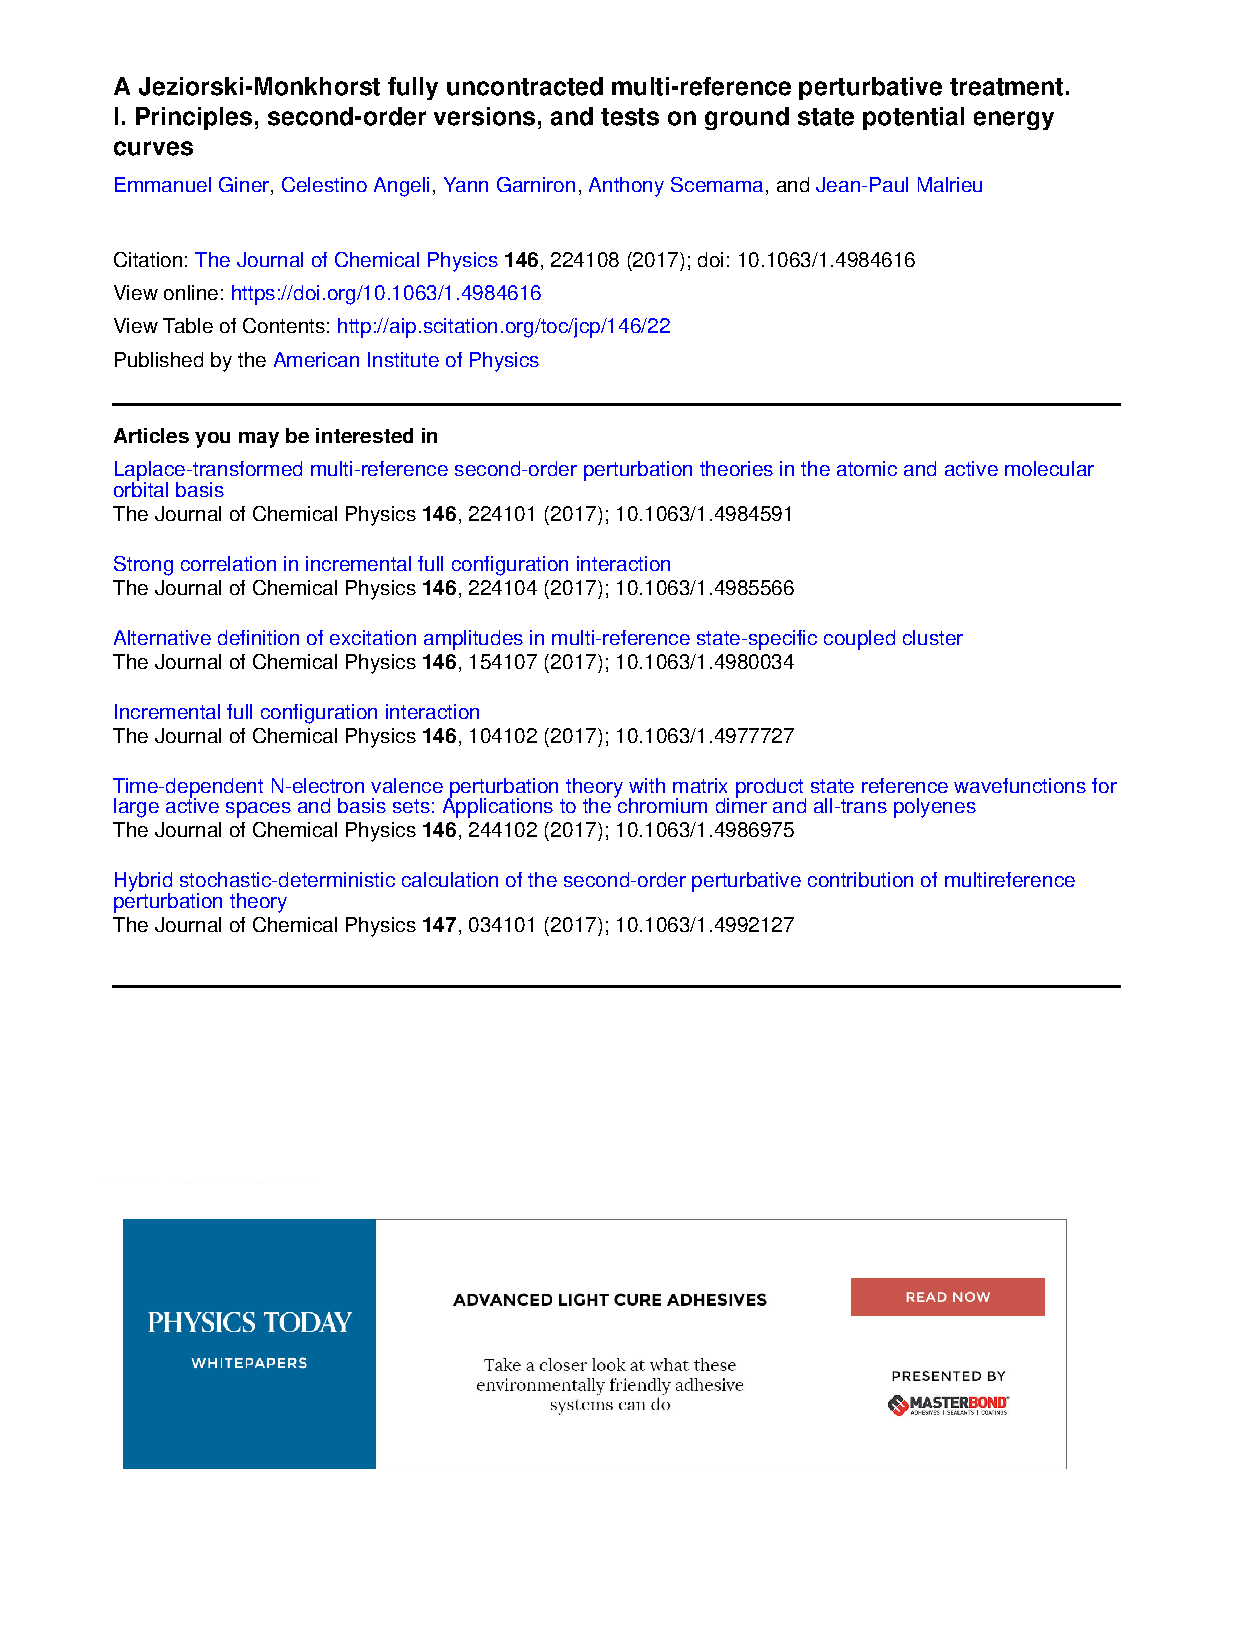
\includepdf[page=2-]{article_jmmrpt2}

\bibliographystyle{ieeetr}
\bibliography{thesis}

%\appendix 
%\chapter{Quantum Package basics}
%\minitoc
%\subfile{qp_general}

\end{document}




